
\usetikzlibrary{arrows.meta,calc,shapes}
\providecommand{\computer}{%
    
\includegraphics[width=1cm]{../common/Noun_project_216.pdf}
}
\providecommand{\switch}{%
    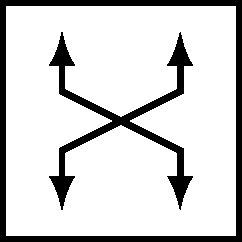
\includegraphics[width=0.9cm]{../common/fig-switch.pdf}
}
\providecommand{\router}{%
    
\includegraphics[width=0.9cm]{../common/fig-router.pdf}
}



\begin{frame}{changing cross-traffic}
\begin{tikzpicture}
\tikzset{
    computer/.style={inner sep=0mm,outer sep=0mm,execute at begin node={\computer}},
    switch/.style={inner sep=0mm,outer sep=0mm,execute at begin node={\switch}},
    router/.style={inner sep=0mm,outer sep=0mm,execute at begin node={\router},circle},
    connect/.style={draw,very thick,Latex-Latex},
    connect big/.style={draw,ultra thick,Latex-Latex},
}
\node[computer] (A) at (0, 0){};
\node[computer] (B) at (13, 0){};
\node[router] (r1) at (5, 0){};
\node[router] (r2) at (10, 0){};
\node[computer] (C) at (3, 3){};
\node[computer] (D) at (12, -3){};
\foreach \x/\y in {A/r1,r1/r2,r2/B,C/r1,r2/D} {
    \draw[connect] (\x) -- (\y);
}
\begin{visibleenv}<2>
\foreach \x/\y in {A/r1,r1/r2,r2/B} {
    \draw[blue,line width=1mm] ([yshift=-1mm]\x) -- ([yshift=-1mm]\y);
}
\node[text=blue,anchor=north] at ([yshift=-3mm]$(A)!0.5!(r1)$) {10Mbit};
\end{visibleenv}
\begin{visibleenv}<3>
\foreach \x/\y in {A.east/r1.west,r1.east/r2.west,r2.east/B.west} {
    \draw[-Latex,blue,line width=1mm] ([yshift=-3mm]\x) -- ([yshift=-3mm]\y);
}
\foreach \x/\y in {C/r1,r1.east/r2.west,r2/D} {
    \draw[-Latex,red,dotted,line width=1mm] ([yshift=3mm]\x) -- ([yshift=3mm]\y);
}
\node[text=blue,anchor=north] at ([yshift=-3mm]$(A)!0.5!(r1)$) {\sout{10Mbit} 7Mbit};
\node[text=red,anchor=west] at ($(C)!0.5!(r1)$) {3Mbit};
\end{visibleenv}
\begin{visibleenv}<4>
\foreach \x/\y in {A/r1,r1/r2,r2/B} {
    \draw[blue,line width=1mm] ([yshift=-1mm]\x) -- ([yshift=-1mm]\y);
}
\node[text=blue,anchor=north] at ([yshift=-3mm]$(A)!0.5!(r1)$) {\sout{10Mbit} \sout{7Mbit} 10Mbit};
\end{visibleenv}
\end{tikzpicture}
\end{frame}

\begin{frame}{adapting to cross-traffic}
    \begin{itemize}
    \item available bandwidth will change
    \item previous example: 3Mbit lost/added from other flow
    \vspace{.5cm}
    \item need to adapt to lost bandwidth
    \item need to detect new available bandwidth
    \end{itemize}
\end{frame}

\begin{frame}{other flow's bandwidth?}
    \begin{itemize}
    \item for now, we'll pretend other flows don't react to us
    \vspace{.5cm}
    \item later topic: what happens when both reacting?
    \end{itemize}
\end{frame}
